\label{sec:eval}

\subsection{실험 환경과 재현성}

모든 실측은 STM32F746G-DISCO 보드(STM32F746NG: Cortex-M7 200MHz
Over-Drive, 단정밀 FPU, I/D 캐시 활성, SRAM 320KB, Flash
1MB)\cite{st_rm0385}에서 수행하였다. 툴체인은 STM32CubeIDE 내장 GNU
Tools for STM32 14.3.rel1(arm-none-eabi-gcc 14.3.1)이며, 네 변형 모두
동일하게 -O3와 LTO, \texttt{ARM\_MATH\_DSP} 조건으로 빌드하였다.
TFLM과 CMSIS-NN은 저장소에 소스로 고정(vendored)하였다 ---
CMSIS-NN은 헤더 기준 리비전 V.12.0.0(2023-09-05), TFLM은 릴리스
태그 없는 업스트림 스냅샷(TFLite 스키마 버전 3)이다.

III장의 대상 모델은 rate 기반 교차 엔트로피 손실(snnTorch
\texttt{ce\_rate\_loss})과 Adam(학습률 $2\times10^{-3}$, 배치 128,
100 에폭)으로 학습하였으며, 학습 로그 정확도는 본 장의 정확도 논의에서
보고한다.

워크로드는 CIFAR-10\cite{krizhevsky2009cifar} 이미지 1장당 rate coding
30 타임스텝($T=30$)이고, 출력 뉴런의 스파이크 값이 $16{,}000$을 넘는
타임스텝을 클래스별로 누적 투표하여 판정한다. 입력 인코딩은 V1만
newlib 표준 \texttt{rand()} 구현이고, V2--V4는 256엔트리 임계값
LUT와 xorshift32(시드 \texttt{0x12345678})를 사용하는 가속 구현이다.
시간은 \texttt{HAL\_GetTick}(해상도 1ms)으로 계측하되, 이미지 1장의
처리 루프 전체(표시 포함)를 total로, 스파이크 인코딩과 신경망 forward의
합을 NN으로 분리 기록하였다. 이미지당 2.4$\sim$9.6초가 소요되므로 1ms
해상도로 인한 상대 오차는 무시할 수 있다. RAM/Flash는 링커 맵과
ST-LINK(HOTPLUG 모드) 판독 기준이다. 변형별 평균에 사용한 이미지 수는
18/16/40/41장으로 이는 측정 세션 길이의 차이일 뿐이며, 분산 데이터는
별도로 저장하지 않았으므로 본 장은 평균값만 보고한다.

비교한 네 변형은 다음과 같다. \textbf{V1}(Scalar): 기준 CHW 스칼라
conv/pool/LIF. \textbf{V2}(TFLM+CMSIS-NN, 비퓨전):
\texttt{CONV\_2D}/\texttt{AVG\_POOL\_2D}/\texttt{FULLY\_CONNECTED}는
빌트인(CMSIS-NN int16x8) 연산자, LIF는 커스텀 SIMD 연산자, 아레나
128KB 설정. \textbf{V3}(제안): 앞 장의 \texttt{SNN\_CONV\_POOL\_LIF}
퓨전 연산자. \textbf{V4}(직접 퓨전): V3와 동일한 퓨전 커널을 TFLM 없이
직접 호출하는 구성(런타임 오버헤드 분리용). 각 변형의 연산자 구성과
아레나 설정은 본 절과 표~\ref{tab:mem}의 명세로 재구성할 수 있다.

\subsection{지연시간}

표~\ref{tab:perf}와 그림~\ref{fig:latency}, \ref{fig:timestep}에
결과를 정리하였다. 핵심 결과는 인코딩$\cdot$LIF$\cdot$런타임 조건이
동일하고 conv/pool 실행 경로만 다른 V2 대 V3 비교로, 제안 퓨전 연산자는
이미지당 $9{,}641.4$ms를 $2{,}407.0$ms로 줄여 \textbf{4.0배}
가속한다. 본 논문의 모든 배속은 이미지당 total 시간 기준이며, NN 시간
기준으로는 V3/V2가 4.10배, V3/V1이 1.89배가 된다.

주목할 실측 발견은 표준 경로의 성능 역전이다. V2는 스칼라
V1($4{,}494.2$ms)보다 오히려 약 2.1배 느리다. 원인은 IV장에서 분석한
커버리지 제약으로, 타임스텝당 MAC의 84\%를 차지하는 conv2(im2col 열
길이 800)가 s16 DSP fast 경로의 적용 조건($<512$)을 위배하여 일반 C
커널로 폴백하기 때문이다. 표준 TinyML 스택을 그대로 적용하는 것이 SNN에서는
최적화가 아니라 감속이 될 수 있음을 보여 주는 결과이다.

V3는 V1 대비로는 종단 1.87배이나, 이 수치에는 V2--V4에만 적용된 입력
인코딩 개선이 포함되므로 커널 효과만의 비교는 대 V2 기준이
공정하다(표~\ref{tab:perf} 각주). 타임스텝당 NN 시간은
147.4/319.0/77.9/77.5ms(V1/V2/V3/V4)이다. 그림~\ref{fig:timestep}에서
보듯 성능의 본질은 퓨전 커널이며, TFLM 런타임의 추가 비용은 V3와 V4의
차이인 이미지당 11.5ms, 약 0.5\%에 불과하다. 즉 해석기 기반 마이크로
런타임의 오버헤드는 SNN의 타임스텝 반복($T=30$회 Invoke)에서도 무시
가능하다.

\begin{table*}[t]
\centering
\caption{네 변형의 실측 성능 비교(이미지당, $T=30$, 동일 -O3+LTO 빌드).}
\label{tab:perf}
\footnotesize
\setlength{\tabcolsep}{4.5pt}
\begin{tabular}{l l r r r r r r}
\hline
변형 & 커널 구성 & total(ms) & NN(ms) & ms/step & 대 V2 & 대 V1 & 이미지 수 \\
\hline
V1 Scalar & 기준 CHW 스칼라, \texttt{rand()} 인코딩 & 4,494.2 & 4,422.7 & 147.4 & 2.15$\times$ & 1.00$\times$ & 18 \\
V2 TFLM+CMSIS-NN(비퓨전) & 빌트인 CONV/POOL/FC + LIF 커스텀 & 9,641.4 & 9,570.0 & 319.0 & 1.00$\times$ & 0.47$\times$ & 16 \\
V3 TFLM+퓨전(제안) & \texttt{SNN\_CONV\_POOL\_LIF} 커스텀 연산자 & \textbf{2,407.0} & 2,335.7 & 77.9 & \textbf{4.0$\times$} & 1.87$\times$ & 40 \\
V4 직접 퓨전(런타임 없음) & 동일 퓨전 커널 직접 호출 & 2,395.5 & 2,324.8 & 77.5 & 4.02$\times$ & 1.88$\times$ & 41 \\
\hline
\end{tabular}
\begin{flushleft}
\footnotesize 주: (a) 모든 배속은 total ms 기준이며, NN 기준으로는
V3/V2 $=4.10\times$, V3/V1 $=1.89\times$이다. (b) V1은 newlib
\texttt{rand()} 인코딩, V2--V4는 LUT+xorshift 인코딩이므로 대 V1
배속에는 인코딩 개선분이 포함된다. 동일 조건 비교는 대 V2이다. (c) V2
감속 원인: conv2의 im2col 열 길이 $5\times5\times32=800$이 CMSIS-NN
s16 DSP fast 경로의 적용 조건($<512$)을 위배하여 일반 C 커널로 폴백.
(d) V3$-$V4 $=$ TFLM 오버헤드 11.5ms(약 0.5\%). (e) ``이미지 수''는 각
변형의 평균 산출에 사용한 이미지 수이며, 차이는 측정 세션 길이에
기인한다.
\end{flushleft}
\end{table*}

\begin{figure}[htbp]
\centering
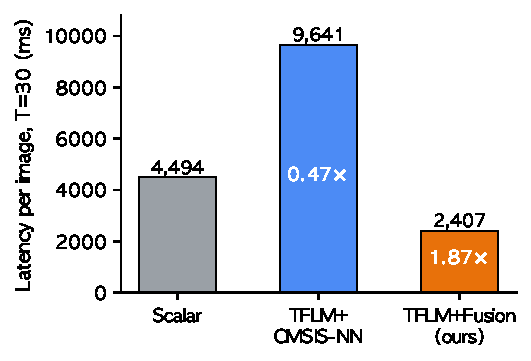
\includegraphics[width=0.86\linewidth]{figures/fig_latency.pdf}
\caption{이미지당 종단 지연시간 실측($T=30$). 막대 안의 배속은 V1
대비이다(V2 0.47$\times$, V3 1.87$\times$).}
\label{fig:latency}
\end{figure}

\begin{figure}[htbp]
\centering
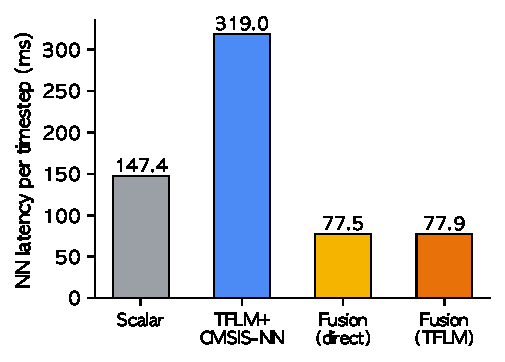
\includegraphics[width=0.86\linewidth]{figures/fig_timestep.pdf}
\caption{타임스텝당 순수 NN 시간. 직접 호출(V4)과 TFLM 통합(V3)의
차이가 TFLM 런타임 오버헤드이다(0.4ms/step, 약 0.5\%).}
\label{fig:timestep}
\end{figure}

\subsection{메모리}

표~\ref{tab:mem}과 그림~\ref{fig:memory}에 변형별 RAM/Flash를
정리하였다. 단위 표기는 본 논문 전체에서 KB는 십진(1,000B),
KiB는 이진(1,024B)이며, 표는 정확한 바이트 값을 병기한다. V3의 Flash $373{,}860$B 중 가중치 계열은
$195{,}328$B(conv1 $6{,}912$B + conv2 $147{,}456$B + FC
$40{,}960$B)이고 나머지 $178{,}532$B가 코드와 런타임이다. 이 분해는
다음 장의 가중치 예산 산술에 사용된다.

V3의 RAM $268{,}200$B는 여유 있게 설정한 256KB($262{,}144$B) 정적
아레나를 포함한 수치이며, 실제 아레나 사용량은
$80{,}288$B($\approx$80.3KB)이다. 같은 커널을 정적 버퍼로 직접
호출하는 V4의 RAM이 $85{,}512$B라는 점이 이 실사용 수치의 하한
근거이며, 아레나 설정값을 줄이면 RAM 총량도 그에 따라 줄어든다. V2는
아레나 $131{,}072$B 설정에 $84{,}544$B를 사용하였다.

\begin{table}[htbp]
\centering
\caption{변형별 메모리 사용(바이트).}
\label{tab:mem}
\footnotesize
\begin{tabular}{l r r r r}
\hline
변형 & RAM & Flash & 아레나 설정 & 아레나 실사용 \\
\hline
V1 & 251,256 & 223,556 & -- & -- \\
V2 & 186,296 & 296,052 & 131,072 & 84,544 \\
V3 & 268,200 & 373,860 & 262,144 & 80,288 \\
V4 & 85,512 & 325,168 & -- & -- \\
\hline
\end{tabular}
\begin{flushleft}
\footnotesize 주: V3의 RAM은 여유 아레나(256KB 설정)를 포함하며, SNN
실소요는 아레나 실사용 80,288B($\approx$80.3KB, 십진 KB)이다.
\end{flushleft}
\end{table}

\begin{figure}[htbp]
\centering
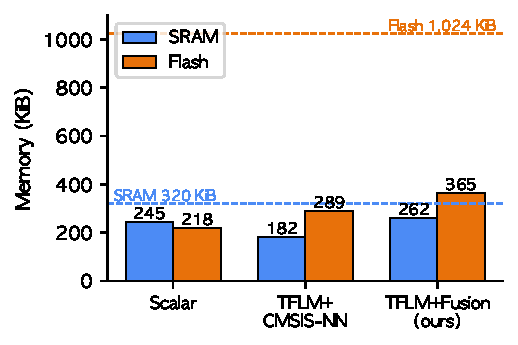
\includegraphics[width=0.86\linewidth]{figures/fig_memory.pdf}
\caption{변형별 SRAM/Flash 사용량과 보드 한계. 그림의 값은
KiB(1,024B) 단위로 본문$\cdot$표의 십진 KB와 환산 기준이 다르다(바이트
값은 표~\ref{tab:mem}). 아레나 없이 정적 버퍼를 쓰는 V4는 그림에서
제외하였다(표~\ref{tab:mem} 참조).}
\label{fig:memory}
\end{figure}

\subsection{수치 정확성 검증}

제안 경로의 정수 산술은 호스트에서 다음 네 단계로 비트 단위 검증하였다.
\begin{enumerate}
\item \textbf{퓨전 항등식}: $6\times6$ 퓨전 가중치의 raw 누산이
  $5\times5$ conv의 4위치 합과 전 픽셀$\cdot$전 채널에서 비트 일치
  --- 식~(\ref{eq:w6}) 변환의 정수 수준 등가 확인.
\item \textbf{커널 대 레퍼런스}: 퓨전 커널과 나이브 레퍼런스 구현을
  30타임스텝$\times$3가지 발화율 입력에서 비교, 스칼라 경로와 SIMD
  경로 모두 비트 일치.
\item \textbf{전체 파이프라인}: TFLM 통합 경로를 독립 레퍼런스와 비교,
  3개 테스트 케이스에서 900개의 출력 스파이크$\cdot$막전위 비트 일치,
  예측 3/3 동일.
\item \textbf{LIF SIMD 전수 검증}: LIF SIMD 커널을
  $1{,}887$만(18.87M) 입력 조합에 대해 스칼라 구현과 전수 비교하여
  비트 일치.
\end{enumerate}

기준 스칼라 경로(V1)와의 비교는 성격이 다르다. 두 경로는 반올림
위치가 다른 정수 구현으로 --- 기준 경로는 시프트 절단과 풀링 반올림의
2회, 퓨전 경로는 requantize 반올림 1회 --- 서로 비트 등가가 아니며, 이 차이로
LIF1 스파이크의 0.75\%가 임계값 근처에서 발화 타이밍이 플립된다.
호스트 3개 케이스에서 최종 예측에는 영향이 없었으며, 본 논문은 두
경로를 통계적으로 등가인 구현으로 서술한다.

\subsection{정확도 수준과 한계}

본 논문의 기여는 정확도 개선이 아니라, 주어진 QAT 모델을 비트
정확하게 그리고 빠르게 배포하는 것이다. 본 모델의 정확도 수준과 그
해석은 다음과 같다.

학습된 QAT 모델의 CIFAR-10 테스트 정확도는 학습 로그 기준으로 배포
체크포인트(에폭 96)에서 50.72\%, 학습 중 최고 51.02\%(에폭 79)였다.
이 수준은 rate coding($T=30$), $94{,}666$개 파라미터의 소형 구조,
per-tensor 8비트 가중치 QAT라는 본 설정의 제약을 반영하는 값이며,
코딩 방식$\cdot$모델 용량$\cdot$학습 기법으로 정확도를 높이는 축은 본
논문의 범위 밖이다.

정수 구현의 정확도는 다음 체인으로 뒷받침된다. (i) 호스트 비트 일치
검증(위 4단계), (ii) 3개 케이스 예측 불변, (iii) 기준 스칼라 경로와의
통계적 등가(0.75\% 타이밍 플립, 예측 불변). (iv) 보조 근거로, 배포
가중치의 정수(Q15) 스칼라 구현은 데스크톱 하니스의 CIFAR-10 학습
분할 100장에서 44/100을 얻는다. 학습 분할의 소표본이라 정식 테스트셋
정확도는 아니나, $n{=}100$의 이항 95\% 신뢰구간(약 $\pm$9.7\%p)에서
QAT 테스트 정확도 50.72\%와 모순되지 않는다. 다만 QAT float
시뮬레이션에서 Q15 정수 구현으로 내려올 때의 정확도 변화 자체는
정량화되지 않았으며, \textbf{정수 구현으로 전체 테스트셋 정확도를
직접 실측하지는 못했다}. 이는 본 논문의 한계이며 향후 과제로 남긴다.

보드에서는 클래스당 1장, 총 10장의 데모 추론을 수행하여 V2가 5/10,
V3가 6/10을 맞혔고, V4의 예측은 V3와 완전히 동일하였다. 표본 10장의
데모이므로 정확도 지표로 해석해서는 안 된다. V2와 V3의 예측은
2장(인덱스 8, 9)에서 서로 다른데, 두 경로 역시 반올림 위치가 다른 정수
구현이다. V2의 표준 경로는 합성곱의 requantize 반올림과 풀링 반올림을
각각 거치며 그 사이에 int16 포화가 개입하는 반면, V3는 requantize
반올림 1회다. 따라서 이 예측 차이는 앞 절에서 관측한 것과 같은 부류의
반올림 경로 차이로 임계값 근처의 발화 타이밍이 달라진 결과로
추정된다(V2--V3 간 스파이크 불일치율은 별도로 측정하지 않았다).
